\documentclass[11pt,dvipsnames,svgnames]{report}

%PRÉAMBULE
\usepackage[french]{babel}
\usepackage[utf8]{inputenc}
\usepackage[table]{xcolor}
\usepackage[T1]{fontenc}
\usepackage[normalem]{ulem}
\usepackage{verbatim}
\usepackage{fancyhdr}
\usepackage{xcolor}
\usepackage{graphicx}
\usepackage{fancybox}
\usepackage{amsfonts}
\usepackage{amsmath}
\usepackage{ulem}
\usepackage{eurosym}
\usepackage{float}
\usepackage{adjustbox}
\usepackage{amssymb,amsmath,latexsym}
\usepackage{mathrsfs}
\usepackage[a4paper]{geometry}
\usepackage[bottom]{footmisc}
\usepackage{perpage}
\usepackage{multicol}
\PassOptionsToPackage{hyphens}{url}
\usepackage[breaklinks]{hyperref}
\usepackage[final]{pdfpages} 
\usepackage{appendix}
\usepackage{caption}
\usepackage{minitoc}
\usepackage{tikz}
\usepackage{setspace}
\usepackage{titlesec}
\usepackage{float}
\usepackage[section]{placeins}
\usepackage{rotating}
\usepackage{subfigure}
\usepackage{epsfig}
%\usepackage{mathpazo}
%\usepackage[scaled]{beramono}
\usepackage{menukeys}
\usepackage{etoolbox}
\makeatletter
\patchcmd{\ttlh@hang}{\parindent\z@}{\parindent\z@\leavevmode}{}{}
\patchcmd{\ttlh@hang}{\noindent}{}{}{}
\makeatother

\geometry{hmargin=2.5cm,vmargin=2cm}



\setcounter{secnumdepth}{4}
\setcounter{tocdepth}{4}


% En-têtes et pieds-de-page
\pagestyle{fancy}
\renewcommand\headrulewidth{1pt}
\fancyhead[L]{\small{\leftmark}}
\fancyhead[R]{
\includegraphics[scale=0.2]{images/logoasi.png}}
\fancyhfoffset{0pt}
\fancyfoot[R]{\setstretch{0,8}\small{GD - AH - MJ - RJ - AL}}
\fancyfoot[L]{
\includegraphics[scale=0.14]{images/LogoINSA.png}}
\renewcommand{\headrule}{{%
 \color{black}\hrule \headwidth \headrulewidth \vskip-\headrulewidth}}
\titleformat{\section}%
[hang]% style du titre (hang, display, runin, leftmargin, drop, wrap)
{\Large\bfseries}%changement de fonte commun au numéro et au titre
{\thesection}% spécification du numéro
{1em}% espace entre le numéro et le titre
{}% changement de fonte du titre


\begin{document}

\begin{titlepage}
\newcommand{\HRule}{\rule{\linewidth}{0.5mm}} 
\center 
\vspace*{\stretch{1}}\textsc{\huge Institut National des Sciences Appliquées de Rouen}\\[0.7cm] 
\LARGE Département ASI~\\[0.5cm]
\Large{Architecture des Systèmes d'Information} ~\\[1.5cm]
\textsc{\Large EC Informatique Répartie}\\[0.5cm] 
\textsc{\large Projet}\\[0.8cm]

\HRule \\[0.4cm]
{ \huge \bfseries Document de Spécifications}\\[0.2cm] \HRule \\[1.5cm]
 
\LARGE \emph{\textbf{Sujet du projet :}} \\
\textbf{Messagerie instantanée et visio/audio-conférence}\\[1.3cm]

\large
	\emph{\textbf{Auteurs :}}\\
	Gautier \textsc{Darchen} \\ 
	Alexandre \textsc{Huat} \\ 
	Marie-Andrée \textsc{Jolibois} \\ 
	Romain \textsc{Judic} \\ 
	Alexandre \textsc{Le Lain}\\[0.3cm]
	\textbf{Étudiants en ASI4}
	
~\\[0.5cm]
\Large \emph{\textbf{Version}}\\
	\textsc{v1.00}
~\\[1cm]

\vfill{\today} 

\begin{figure}

\includegraphics[width=4cm]{images/LogoINSA.png}\hfill

\includegraphics[width=3cm]{images/logoasi.png}
\end{figure}

%----------------------------------------------------------------------------------------

\vspace*{\stretch{1}} 
 \end{titlepage}

\newpage
\tableofcontents

\newpage


\chapter{Introduction}

L'application à développer est une plateforme de messagerie instantanée entre deux interlocuteurs. Elle permettra à ces interlocuteurs de communiquer tout en étant connectés sur des machines distantes. 


\section{Fonctions principales}
Les fonctions principales de cette application peuvent être scindées en trois catégories : 
D'une part, \textbf{l'échange de message}, d'autre part, \textbf{ le filtrage des messages en fonction de leur contenu}, \textbf{l'utilisation d'un avatar}.

Concernant la première fonctionalité, les interlocuteurs pourront s'envoyer des messages écrits de façon instantanée. Ils auront en plus la possibilité de communiquer avec d'autres formats via un système de visio ou audio-conférence intégré à l'application.

Concernant le filtrage des messages, il concernera le contenu et permettra deux sous-fonctionnalités, à savoir le contrôle parental et la modération. Les utilisateurs auront la possibilité de choisir d'activer ou non ce système de filtrage. De plus ce dernier pourra être personnalisé.

Concernant la dernière fonctionalité, un système d'avatar pourra être utilisé par les utilisateurs dans différents cas (absence d'une webcam ou encore lors d'une discussion en messages écrits).


\section{Utilisateurs}
L'application pourra fonctionner si un seul ou plusieurs utilisateurs humains sont connectés :
\begin{itemize}
\item \textbf{Humain utilisateur : } capable de créer une conversation, de participer à une conversation qu'il sélectionne, d'envoyer des messages et de dialoguer via audio ou visio conférence. L'utilisateur peut choisir ses données de pramétrages de filtrage. A la connexion il choisit aussi un login et une image.
\item \textbf{Humain administrateur flitrage} Peut supprimer un message qu'il n'a pas émis. L'analyser le filtrer et générer un message générique expliquant la modération.
\end{itemize}
\vskip \baselineskip

Pour utiliser l'application, les utilisateurs devront simplement avoir les compétences informatiques de base (se connecter à internet, utiliser une plateforme en ligne...).

\chapter{Besoins détaillés}
\section{Spécifications fonctionnelles}
\subsection{Cas d'utilisation}
\begin{figure}[H]
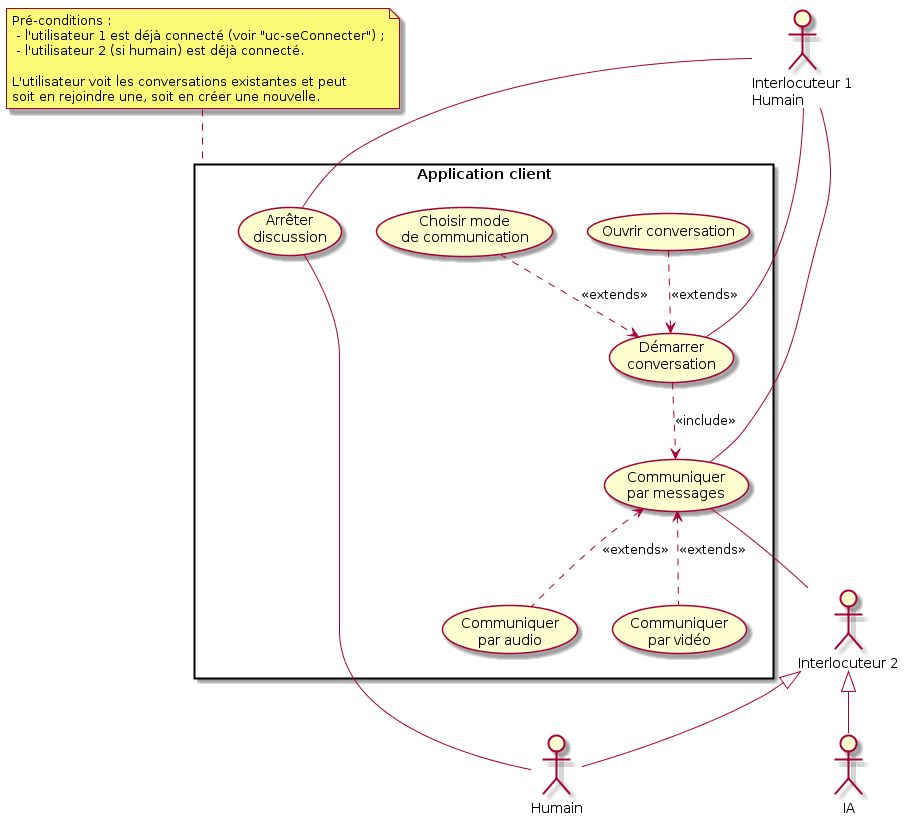
\includegraphics[scale=0.55]{images/uc-discuter.png}
\caption{Cas d'utilisation \textbf{discuter}}
	Ce cas d'utilisation représente les interactions entre les différents interlocuteurs ( Humain et IA ) et les différents moyens mis à leur disposition pour effectuer cette action.
\end{figure}

\begin{center}
\begin{figure}
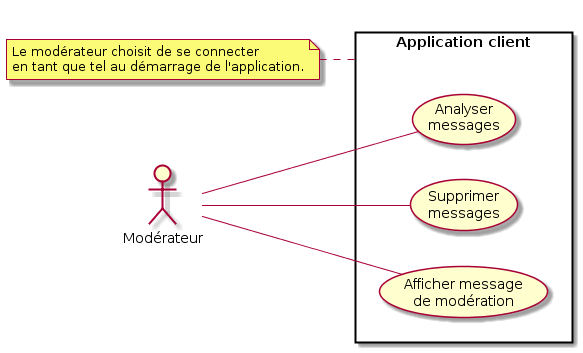
\includegraphics[scale=0.7]{images/uc-filtrerMessages.png}
\vspace{5\baselineskip}
\caption{Cas d'utilisation \textbf{filtrer les messages}}	
	Ici, le cas d'utilisation indique qu'un utilisateur possédant le rôle de modérateur est en mesure de filtrer des conversations (Analyse des messages, suppression de messages ne respectant pas le filtre choisi par le modérateur,...).
\end{figure}

\begin{figure}
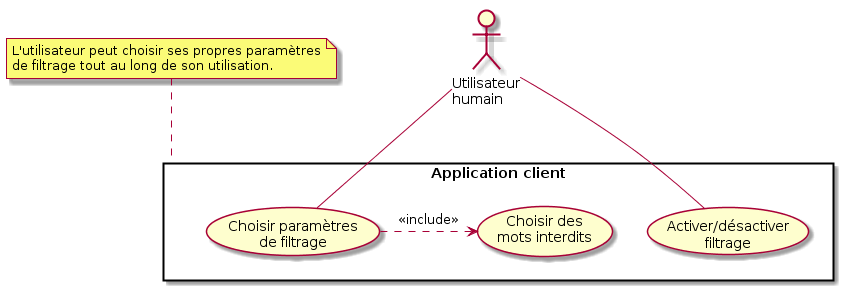
\includegraphics[scale=0.6]{images/uc-parametrerFiltrage.png}
\caption{Cas d'utilisation \textbf{paramétrer le filtrage}}
	Dans la continuation du cas d'utilisation précédent, l'utilisateur peut choisir d'appliquer ou non des filtres à ses conversations en fonctions de différents paramètres.
\end{figure}

\begin{figure}
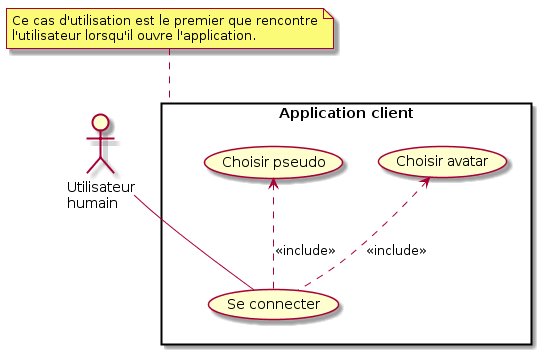
\includegraphics[scale=0.7]{images/uc-seConnecter.png}
\caption{Cas d'utilisation \textbf{se Connecter}}
	Ce cas d'utilisation représente l'action "se Connecter" qui permet à l'utilisateur d’accéder aux services de l'application.
\end{figure}

\end{center}

\section{Spécifications d'interfaces}
\subsection{Maquettes}
\begin{center}
\begin{figure}
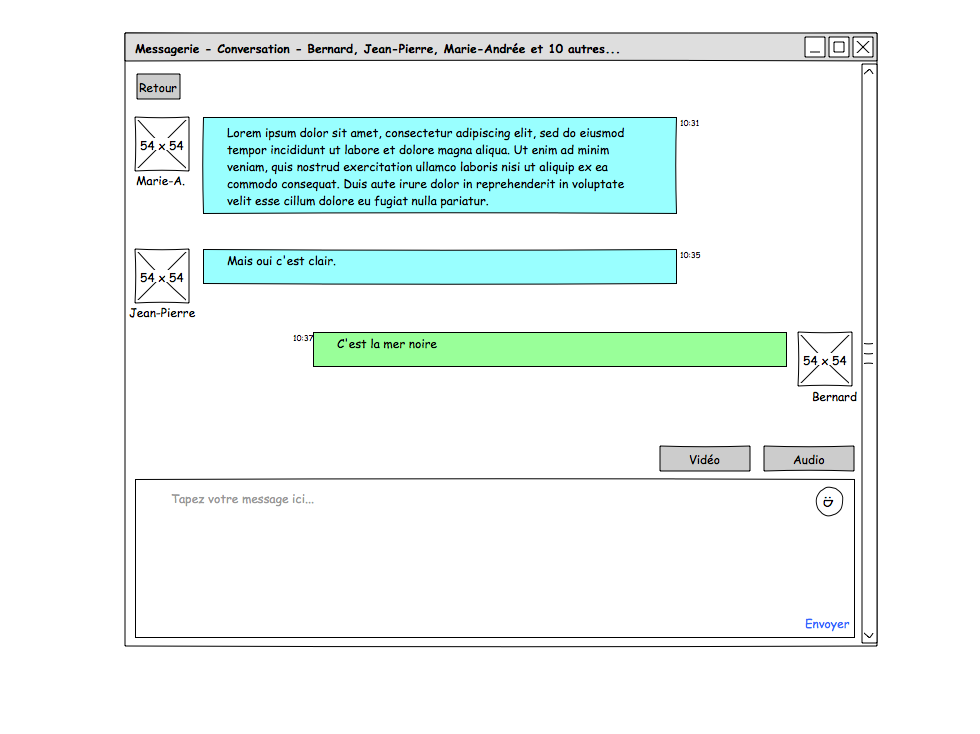
\includegraphics[width=\textwidth]{maquette/maquette1.png}
\caption{\textbf{Un exemple de conversation}}
\end{figure}

\begin{figure}
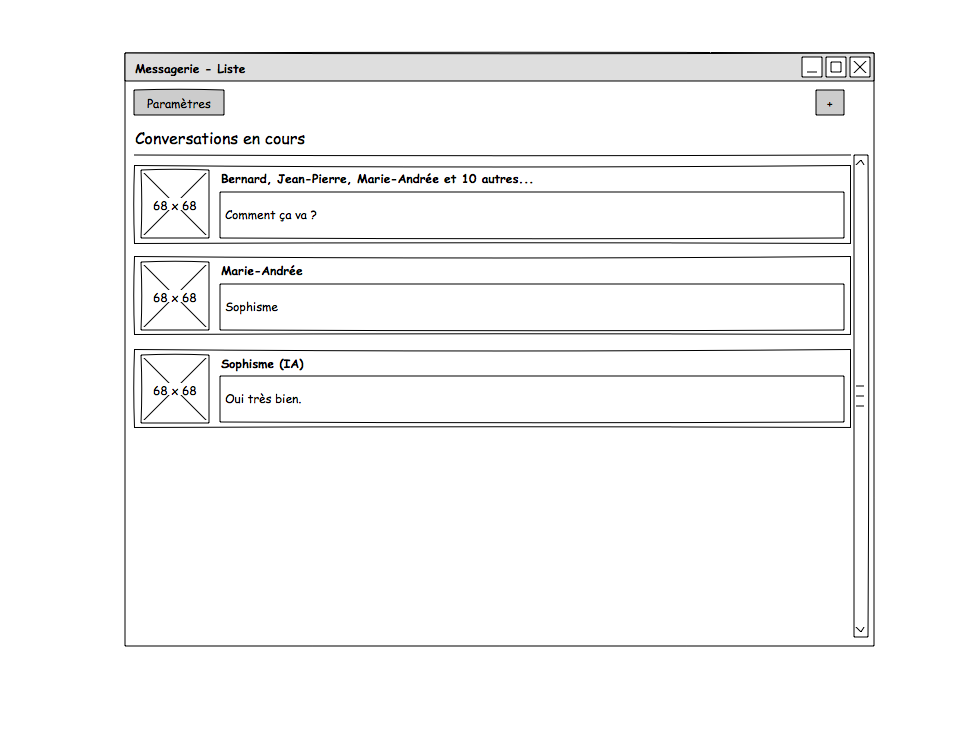
\includegraphics[width=\textwidth]{maquette/maquette2.png}
\caption{\textbf{Autre exemple de conversation}}
\end{figure}

\begin{figure}
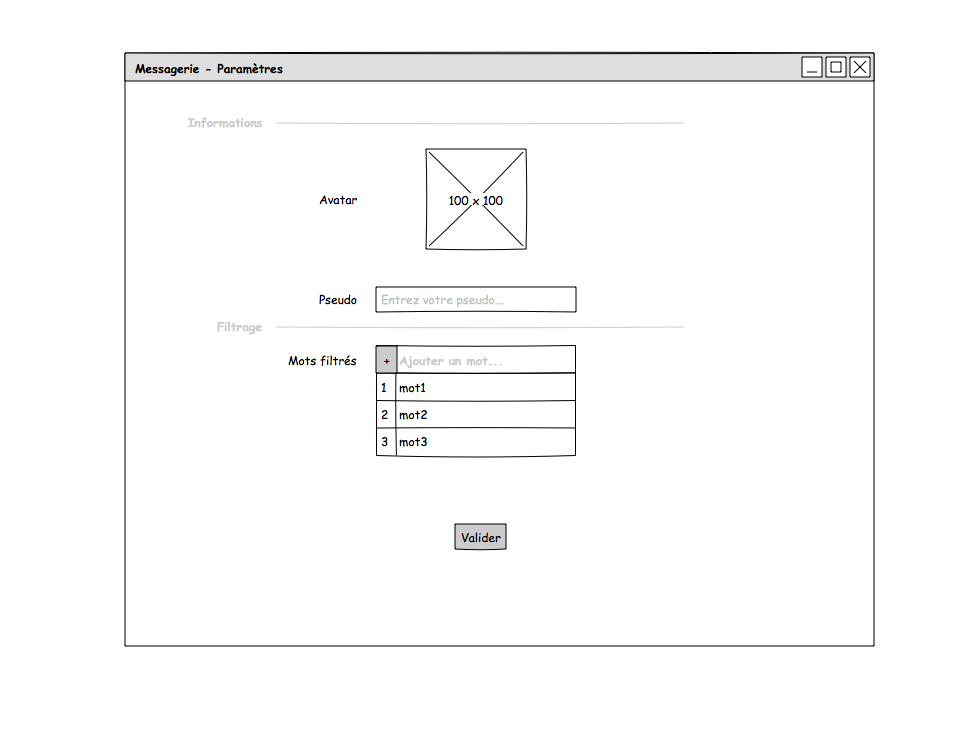
\includegraphics[width=\textwidth]{maquette/maquette3.png}
\caption{\textbf{Interface des paramètres}}
\end{figure}
\end{center}


\section{Spécifications opérationnelles}

\chapter{Contraintes}
\section{Contraintes matérielles}
L'application est accessible en ligne car elle est hébergée sur un serveur. De ce fait, l'utilisateur doit de disposer d'une machine reliée à internet.

Pour profiter du service visio, l'utilisateur doit posséder un matériel de capture vidéo (webcam).

Pour utiliser le service audio, l'utilisateur doit posséder une entrée et une sortie audio.

La majorité des calculs est réalisée côté serveur, ce qui n'implique pas un besoin de ressources conséquent côté client.

\section{Contraintes logicielles}
L'application sera hébergée sur un serveur distant.
Pour utiliser l'application il est nécessaire d'être connecté à internet, de plus le serveur qui héberge l'application doit tourner.


\end{document}